% TEMPLATE for Usenix papers, specifically to meet requirements of
%  USENIX '05
% originally a template for producing IEEE-format articles using LaTeX.
%   written by Matthew Ward, CS Department, Worcester Polytechnic Institute.
% adapted by David Beazley for his excellent SWIG paper in Proceedings,
%   Tcl 96
% turned into a smartass generic template by De Clarke, with thanks to
%   both the above pioneers
% use at your own risk.  Complaints to /dev/null.
% make it two column with no page numbering, default is 10 point

% Munged by Fred Douglis <douglis@research.att.com> 10/97 to separate
% the .sty file from the LaTeX source template, so that people can
% more easily include the .sty file into an existing document.  Also
% changed to more closely follow the style guidelines as represented
% by the Word sample file.

% Note that since 2010, USENIX does not require endnotes. If you want
% foot of page notes, don't include the endnotes package in the
% usepackage command, below.

% This version uses the latex2e styles, not the very ancient 2.09 stuff.

%%%%%%%%%%%%%%%%%%%%%%%%%%%%%%%%%%%%%%%%%%%%%%%%%%%%%%%%%%%%%%%%%%%%%%
%  Packages
%%%%%%%%%%%%%%%%%%%%%%%%%%%%%%%%%%%%%%%%%%%%%%%%%%%%%%%%%%%%%%%%%%%%%%


\documentclass[letterpaper,twocolumn,10pt]{article}
\usepackage{usenix,epsfig,endnotes}
\usepackage{url}
\usepackage{multirow}
\usepackage{booktabs}
\usepackage{color}
\usepackage[normalem]{ulem}
\usepackage[usenames,dvipsnames]{xcolor}
\usepackage{pifont}
\usepackage{graphicx}
\usepackage{makecell}
\usepackage{enumitem}
\usepackage{xspace}


\newcommand{\urlwofont}[1]{\underline{\urlstyle{same}\url{#1}}}
\newif\ifrev
%  COMMENT OUT NEXT LINE TO HIDE TODOs AND COMMENTS
\revtrue

\newcommand{\lip}{\emph{Lock-in-Pop}\xspace}
\ifrev
  \newcommand{\brendan}[1]{{\color{purple} [Brendan: #1]}}
  \newcommand{\yanyan}[1]{{\color{blue} [Yanyan: #1]}}
  \newcommand{\cappos}[1]{{\color{red} [Justin: #1]}}
  \newcommand{\lois}[1]{{\color{magenta} [Lois: #1]}}
  \newcommand{\yiwen}[1]{{\color{OliveGreen} [Yiwen: #1]}}
  \newcommand{\todo}[1]{{\color{Orange} [TODO: #1]}}
\else
  \newcommand{\brendan}[1]{}
  \newcommand{\yanyan}[1]{}
  \newcommand{\cappos}[1]{}
  \newcommand{\lois}[1]{}
  \newcommand{\yiwen}[1]{}
  \newcommand{\todo}[1]{}
\fi

\setlist[itemize]{leftmargin=*}

\begin{document}


%don't want date printed
%\date{}


%%%%%%%%%%%%%%%%%%%%%%%%%%%%%%%%%%%%%%%%%%%%%%%%%%%%%%%%%%%%%%%%%%%%%%
%  Title and Authors
%%%%%%%%%%%%%%%%%%%%%%%%%%%%%%%%%%%%%%%%%%%%%%%%%%%%%%%%%%%%%%%%%%%%%%


%make title bold and 14 pt font (Latex default is non-bold, 16 pt)
\title{\Large \bf{Lock-in-Pop: New Design Secures Privileged Operating System Kernels by Keeping on the Beaten Path}}


%for single author (just remove % characters)
%\author{
%{\rm Yiwen Li}\\
%New York University \\
%liyiwen@nyu.edu
%\and
%{\rm Ali Gholami}\\
%KTH Royal Institute of Technology\\
%gholami@kth.se
%\and
%{\rm Chris Matthews}\\
%Apple Inc. \\
%chris.matthews@apple.com
%\and
%{\rm Yanyan Zhuang}\\
%New York University \\
%yyzh@nyu.edu
%\and
%{\rm Justin Cappos}\\
%New York University \\
%jcappos@nyu.edu
%} % end author


\maketitle


% Use the following at camera-ready time to suppress page numbers.
% Comment it out when you first submit the paper for review.
\thispagestyle{empty}



%%%%%%%%%%%%%%%%%%%%%%%%%%%%%%%%%%%%%%%%%%%%%%%%%%%%%%%%%%%%%%%%%%%%%%
%  Sections
%%%%%%%%%%%%%%%%%%%%%%%%%%%%%%%%%%%%%%%%%%%%%%%%%%%%%%%%%%%%%%%%%%%%%%


\subsection*{Abstract}
%A possible compromise of privileged code, such as that in the OS kernel, is a
%daunting security threat. Severe vulnerabilities discovered in this code
%have resulted in privilege escalation, denial of service, memory corruption and
%other complications. 
Virtual machines are widely used in practice, in part for their ability to
isolate potentially untrusted code from the rest of the system.
%Virtual machines have been developed to protect kernel code
%through isolation. 
However, it is often possible to trigger zero-day flaws
in the host OS kernel from inside of a guest OS VM.  %Thus, the current 
%manner of constructing OS VMs does not provide strong resilience 
%Yet, when running it is possible to exploited in a number of VMs, indicating
%that isolation alone is not sufficient protection. 
In this paper, we use an observation about where security bugs lie to
devise a new design model that improves the security of applications
run in OS VMs.  %document the development of a different type of virtual
%machine to secure the OS kernel. 
We begin by observing that a portion of the OS kernel (those kernel paths used 
by popular applications in everyday use) contain fewer security bugs. We 
leverage this knowledge to devise a novel design called Lock-in-Pop, which 
locks an application (and the POSIX implementation that services it) into only 
accessing that portion of the kernel.  Using the Lock-in-Pop model, we 
implement a virtual machine called Lind.
%a very small trusted computing base. Complex functionalities in Lind are performed
%within a sandbox, using a memory-safe programming language to re-create riskier system calls.
We took the versions of Lind and seven other virtualization systems that were
available at the release of Linux kernel version 3.14.1 and evaluated
their effectiveness containing the zero day kernel bugs that were discovered 
since then.
%against zero day
%bugs discovered in the Linux kernel version 3.14.1.
%When Lind was tested against seven other virtual machines to see whether it would
%   trigger any of 35 bugs examined in Linux kernel version 3.14.1, the threat of
%    an attack was reduced to less than 3\%. 
Our results show it is substantially harder to trigger zero day bugs in 
Lind (3\%) than existing systems like VirtualBox (40\%), VMWare Workstation
(31\%), Docker (23\%), LXC (34\%), QEMU (14\%), KVM (14\%), and Graphene (23\%).

\section{Introduction}
\label{sec.introduction}

For many years system designers and developers have had to deal with a common security issue --
how to defend against threats hidden within the system's own code. Despite
 decades of effort, researchers still frequently uncover new flaws in operating
 system kernels. Such flaws are dangerous because, if triggered by an untrusted
 program, these bugs can lead to security threats like privilege escalation
 [CVE-2016-0728], [CVE-2015-8660], denial of service [CVE-2015-8539], [CVE-2015-5364],
  and memory corruption [CVE-2014-9529].

The search for an ideal way to protect kernel code has been hampered by limited
knowledge of the security impact of its interaction with user programs.
A number of strategies have been attempted. One prevailing belief was that virtual
machines could provide enough isolation to execute programs safely.
However, when Virtualbox reports 40 vulnerabilities \cite{Virtualbox-Vulnerabilities},
 and more than 100 bugs have been found in VMware Workstation,
it suggests that isolation alone may not be enough. Other researchers have looked
 to the development of metrics capable of pinpointing bugs, and, therefore,
securing the most vulnerable areas\cite{PittSFIeld, ozment2006milk}. As these
examples indicate, the design of secure systems has been somewhat “hit-or-miss.”
 Observations may lead to
 the reduction of specific threats, but not to a reproducible, broadly applicable,
quantitative design solution.

With this paper, we move one step closer to identifying such a solution. We start
 with the proposition that code found in popular paths, associated with frequently-used programs,
has less potential risk of bugs than code in less-used parts of the kernel.
Therefore, we will be able to determine which lines of code can be executed
 safely within the OS kernel. We performed a quantitative analysis of resilience
  to flaws in two versions of the Linux kernel, and
found that only 2.5\% - 4.0\% of the bugs were present in popular code paths,
despite these paths accounting for nearly 32.2\% - 34.5\% of the total reachable kernel code.
When we ran the same study on the same Linux kernel versions using two other metrics
(Chou \cite{PittSFIeld} and Ozment \cite{ozment2006milk}),
we found them less effective at predicting the location of zero-day bugs in the
Linux kernel versions that we tested.

Guided by this knowledge, we propose a new design scheme for a secure virtual machine that
accesses only the popular code paths through a very small trusted computing base.
We gave it the name \emph{Lock-in-Pop}, because it locks out kernel access to all code except
that found in paths associated with frequently-used popular programs. The design
requires an interface built only on basic OS primitives. This is sufficient to
perform operations for file systems, such as
networking, threading, memory management, and other required functions.
For complex functionalities,  \emph{Lock-in-Pop} re-creates system calls in
a memory-safe programming language sandbox.

To demonstrate the viability of \emph{Lock-in-Pop} we use it to implement a new
prototype virtual machine that can offer enhanced security without sacrificing
 basic functionality. Dubbed Lind, it pairs two components -- Google's Native Client
(NaCl) and Seattle's Repy. NaCl serves as a computational module that isolates
binaries, providing memory
safety for a legacy program like Apache. It also passes system calls invoked by
the program to the operating system interface, called SafePOSIX. This interface,
isolated within the Repy
sandbox, ensures access to only popular paths. However, the small (8K LOC) sandbox
kernel allows complex operating system functionalities to be built on top of the machine.

To test Lind's effectiveness, we replicated 35 kernel bugs in the Linux kernel
version 3.14.1,
and attempted to trigger them in seven other virtualized environments,
including VirtualBox, VMWare Workstation,
Docker, LXC, KVM, QEMU, and Graphene.
Our results show that applications in Lind were the least likely to trigger kernel bugs,
with only one out of the 35 (2.9\%) kernel vulnerabilities tested for being triggered.

In summary, the main contributions of this paper are as follows:

\begin{itemize}\setlength\itemsep{0em}
\item
We postulate a new approach for securing privileged code,
such as the OS kernel, based on the idea that popular kernel paths contain fewer bugs.

\item
We propose a quantitative metric that evaluates security
 at the lines-of-code level.
After testing this metric against others, we find it effective in locating
 bugs in the Linux kernel.

\item
Based on the metric, we develop a new design scheme called \emph{Lock-in-Pop} that
accesses only popular code paths
through a very small trusted computer base.
The need for complex functionality is addressed by re-creating riskier systems calls
in a memory-safe programming language within a secure sandbox.

\item
We build a prototype virtual machine, Lind, using the \emph{Lock-in-Pop} design,
 and test its effectiveness against seven other security systems. We find that
 Lind triggers only one
(2.9\%) of the 35 zero day bugs we had targeted,
making it an order of magnitude more secure than other systems.
\end{itemize}

%\yiwen{Can we lose the last map paragraph? I'd like to remove it and it will save a lot of space.}
%
%The remainder of this paper is organized as follows.
%Section \ref{sec.motivation-and-background} presents the scope of our study and our threat model.
%A study of earlier kernel protection metrics and the results of tests we ran to compare their performance
%against our newly proposed design are discussed in Section \ref{sec.metric}.
%Section \ref{sec.design} describes the development of our \emph{Lock-in-Pop} design scheme.
%In Section \ref{sec.implementation} we discuss the construction of the Lind prototype,
%while Section \ref{sec.evaluation} provides the  results of tests that directly compare Lind's performance
%in preventing the triggering of bugs to other virtualization systems.
%Section \ref{sec.limitation} outlines possible future initiatives.
%Finally, Section \ref{sec.related_work} reviews existing design metrics, as well as techniques that share some of Lind's security techniques and goals,
%while the cogent points relayed in the paper are reviewed in Section \ref{sec.conclusion}.

\section{Goals and Threat Model}
\label{sec.motivation-and-background}

\textbf{Goals.}
Our goal is to design and build a secure virtualization system that allows
untrusted programs to run on an unpatched and vulnerable host OS (Linux OS in
this study), without triggering vulnerabilities that attackers could exploit.
Developing effective defenses for the host OS kernel is essential as kernel code
can expose privileged access to attackers that could lead to a system take-over.

To combat this threat, untrusted programs are often executed in a 
secure virtualization system, such as a guest OS virtual machine, a system call 
interposition module, or a library OS system. Our intent is to
build such a system capable of protecting not only
an underlying host OS, but also any programs running in it, from both 
malicious attacks
and accidental triggering by applications.  \cappos{I do not know what
you mean to convey with the previous sentence.}
In this section, we define the scope of our efforts. We also briefly note why 
this study does not evaluate a few existing design schemes.

\cappos{This paragraph also is confusing to me.}
\yanyan{please check my edits.}
%We start by acknowledging that 
It is possible for an attack attempt to be staged
on a host OS in a secure virtualization system.
Furthermore, %we anticipate that 
such an exploit could be done directly or indirectly.
In a direct exploit, the attacker can access a portion of host OS's kernel
that have a vulnerability. In an indirect exploit,
the attacker takes advantage of a vulnerability in the virtualization system to 
run arbitrary code, escapes the VM's containment and can 
make system calls into the host OS. 
The secure virtualization system design we will propose
in Section~\ref{sec.design} is designed to prevent both types of attacks.

\noindent
\textbf{Threat model.}
Based on the goals mentioned above, we make the following assumptions about the
potential threats our system could face:

\begin{itemize}\setlength\itemsep{0em}

\item The attacker possesses the knowledge about one or more unpatched 
vulnerabilities in the host OS.

\item The attacker is permitted to execute any code in the secure 
virtualization system.

\item If the attack program can trigger a vulnerability in any privileged 
code, whether in the host OS or the secure virtualization system, the attacker 
is then considered successful in compromising the system.

\end{itemize}

\noindent
\textbf{Exclusion.}
It should be noted that our study intentionally excludes %several existing
%approaches to virtualization systems. We considered these techniques
%out of scope due to differences in hardware and software requirements.
%Primarily we chose to exclude 
a comparison with solutions that do not run on top of on a 
full-fledged privileged operating system, such as a virtualization system that 
uses a bare-metal hypervisor~\cite{Xen-03, VMWare-Server} or 
hardware-based virtualization solution~\cite{IntelVT, keller2010nohype}. 
While the ideas and techniques we apply here potentially apply to those 
systems, a direct comparison is not possible since they have different
trusted computing bases.
%would be difficult to perform due to 
%tracing techniques.
%These devices are dependent on the underlying hardware, and do not interact
%with a privileged OS kernel. Such differences in both structure and function
%make it difficult to directly compare these techniques to our proposed model.

To build a system to resist zero-day vulnerabilities, we need to know what
portions of the kernel may be more prone to exploitation. Our first step is to
define and test a security metric that can quantitatively measure how bugs and
vulnerabilities are distributed in the kernel.

\section{Developing and Assessing a Quantitative Evaluation Metric for Kernel Security}
\label{sec.metric}
%\cappos{possible intro sentence / paragraph...}
As mentioned in the previous section, there has been a lack of reliable quantitative
metrics for the development of kernel security systems. Therefore, our first step
was to develop a quantitative metric that could more accurately identify portions of
the OS kernel that had the highest potential to unleash inherent bugs begins with a
hypothesis based on observation and common sense. In this section, we show how we
went about documenting the accuracy of the statement below.

kernel paths that are executed by common applications
during everyday use are less likely to contain security flaws.

This key hypothesis posits that by understanding how and when
a line of code in the kernel is used, we can predict its likelihood to
contain a security flaw.
The intuition is that these code paths are very well-tested
due to their constant use, and thus it is much less likely that security bugs
will occur in these lines of code.
%Since there are relatively few security
%bugs disclosed (dozens) compared to the total number of lines of kernel
%code (millions),

%To test this hypothesis we conducted the following experiment.



%The first step to addressing the threat articulated above is to establish metric
%by which kernel security can be quantitatively evaluated. In this section
%we document the development of such a metric.
%First, we look at current commonly used metrics for code complexity and why they may be less than effective.
%The next section discusses our proposed metric, which focuses on using the kernel code paths accessed by widely used applications.
%Finally, we use the metric to verify our central hypothesis, by testing for the presence of 40 severe Linux  Kernel bugs.

%\lois{This intro section needs work. I'm not happy with what is  here, though I think it is somewhat clearer than what was there before.}

%Before a metric can be developed to meet the threat outlined in Section 2, we need to
%establish a better understanding of basic kernel behavior, and review what we know about
%the risk inherent in privileged code. This section briefly touches on past risk
%metrics, as well as the key hypothesis used to guide the capture and evaluation
%of kernel traces in our study.




%\subsection{Key Hypothesis}
%
%Our metric development begins with the positing of a hypothesis
%that kernel paths executed by popular applications, such as Web browsers or
%text editors, are likely to contain fewer exploitable bugs than uncommonly used paths.
%As they are frequently used, bugs and vulnerabilities in these common kernel
%paths are more likely to have been caught by developers.
%
%In putting forth this hypothesis, we narrow our ``common paths" definition
%to also exclude widely used system calls if they include rare arguments
%and flags. The proposed metric also excludes odd execution paths through popular
%system calls.

\subsection{Experiment Setup}

To test our hypothesis we performed an analysis of two different versions of
the Linux kernel, 3.13.0 and 3.14.1.  Our findings for these
versions are quantitatively and qualitatively similar, so we report
the results for 3.13.0 in this section and use 3.14.1 in Section~\ref{sec.evaluation}.
%\cappos{Fix the version here please.}
To trace the kernel, we used \texttt{gcov}~\cite{gcov}. A standard utility with
the GNU compiler collection (GCC) suite,
\texttt{gcov} is a program profiling tool that indicates which lines of kernel
code are executed while an application runs.

\textbf{Commonly-used kernel paths.}
To capture the commonly-used kernel paths, we used two strategies concurrently.
First, we attempted to capture the normal usage behavior of popular applications.
To do this, two students used
applications in the 50 most popular Debian packages~\cite{Top-Packages}
(omitting libraries) for Debian 7.0.
%Since many such packages are libraries that other programs
%depend on, this resulted in using 50 \cappos{Exactly 50?} \yiwen{Yes. Exactly 50. We chose to stop when we have 50 of them working.} applications.
Each student used 25 applications for their designed
tasks (i.e., writing, spell checking, and then printing a letter in a text
editor, or recoloring and adding a caption to a picture in image processing
software). In instances where there were two applications that performed a
similar task (i.e., Mozilla Firefox and Google Chrome), both programs were
used. These tests were completed over 20 hours of
total use over 5 calendar days.
%\cappos{Were the results the same for the two students?  What percent of LOC varied?}

The second strategy was to try to capture the total range of usages for a
specific computer user. Hence the students used the workstation as their
desktop machine for a one week period. They did their homework, developed
software, communicated with friends and family, etc., using this system.
Software was installed as needed.

Using these two strategies, we obtained a profile of the lines of
kernel code (publicly available at~\cite{Lind}), that indicate
a set of commonly-used kernel paths.

%\cappos{What does the following text actually mean?}
%\yiwen{The following file system operations should belong to the second strategy about
%uses for a specific computer user. The student performed file system operations, like creating
%a folder, deleting a file, etc. during his daily use of the computer, which is part of our test.}
%Several other operations needed to access common paths were conducted, including
%intensive file management tasks to create/read/update or delete files and
%directories from the underlying filesystem.

%The first step in proving our hypothesis was to capture the lines of kernel
%code executed when running applications.
%The OS kernel code
%is organized under different kernel directories.
%Whenever an application tries to access system resources, such as file
%system, I/O and memory, the kernel code under the corresponding paths is executed. Therefore,
%its code execution reflects the basic behavior of the kernel, in response
%to user application requests. To better understand this, we identified and
%captured which lines of code in the kernel
%were executed when running a user program, and named them  \textit{kernel traces}.
%Because these traces are closely related to the program that generates them, it is
%possible to compare different security systems.
%To capture kernel traces, we used \texttt{gcov} \cite{gcov}, a program profiling
%tool that is a standard utility with the GNU compiler collection
%(GCC) suite.

\textbf{Locating bugs.}
Having identified the kernel paths used during application execution, we next
addressed how bugs are distributed in these paths. We collected a list of
severe kernel bugs from the National Vulnerability Database~\cite{NVD}.
%the U.S. government repository of standards-based vulnerability management
%data~\cite{NVD}.
For each bug, we
found the patch that fixed the problem and identified
which lines of kernel code were modified to remove the bug.
For the purpose of this study, a user program that can execute a line of kernel
code changed by such a patch is considered to have the \textit{potential to
exploit that flaw}.  Note, it is possible that in some situations this may
overestimate the ability for an attacker to exploit a flaw, since it may be
possible that additional lines of code must also be executed.


%We determined that any lines of code in the kernel would be considered risky
%if they triggered one or more vulnerability. Other lines of code
%that did not trigger a vulnerability would be considered to be safe to access.
%These lines of code would then compose the common (or safe) portion of the kernel,
%which can be trusted to build a secure trusted computing base for secure systems.
\subsection{Results and Analysis}
\label{Verification-of-Hypothesis}


%To test the hypothesis that commonly used kernel paths contain fewer bugs, we needed
%to identify these paths as a subset of the total reachable kernel paths.
%
%\textbf{Total Reachable Kernel Paths}
%The next step was to obtain the total reachable paths and then analyze the location of
%any vulnerabilities. To accomplish this, we conducted two separate operations.
%
%\begin{enumerate}
%During this step, we conducted

%\textit{System Call Fuzzing}
%System call fuzzing experiments were designed to utilize the Trinity
%system call fuzz tester~\cite{Trinity}. These included sequential execution of
%more than 300 system calls with 1 million iterations
%for executing each system call by 16 child processes (Trinity workers).
%The obtained kernel trace comprehensively reflected various aspects of the
%kernel functionalities.

%\textit{Linux Test Project}
%Linux Test Project (LTP) \cite{LTP} is another tool to generate the kernel traces
%for running all the available system call in different scenarios.
%By using LTP we could validate the kernel traces that
%were generated by Trinity or catch the possible traces that were missing.
%
%\textbf{CVE Bug Reports}
%The last test needed to verify our hypothesis was to check which portions of
%the kernel contained bugs. This was accomplished done by comparing the kernel
%traces with the lines of code we labeled for each bug, based on change of lines in the
%kernel patch. We examined 40 severe Linux kernel
%bugs that had been discovered by the research community in the last five
%years (represented by the first two columns in Table
%\ref{table:vulnerabilities_commonly_used_kernel_paths}).
%The bugs chosen from the NVD bug database have the highest severity score.
%
%\subsubsection{Results and Evaluation}
We now examine our hypothesis given traces for the commonly-used kernel
paths and the set of lines that were patched to fix bugs. We found that
only one of the 40 kernel bugs falls within the commonly-used paths, despite
the commonly-used kernel paths making up 12.4\% of the kernel.
To verify that bugs are more likely to appear in certain parts of
the kernel, we performed the following analysis.

%\cappos{Draft statistical analysis text from Dan.  Needs work...}
We assume that kernel bugs appear at an average rate proportional to the
number of lines of kernel code, and independently of the time since the last
bug occurrence. Therefore, the rate of defect occurrence per LOC
follows a Poisson distribution~\cite{Poisson-distribution}.
%For analysis, we chose to model the rate of defect occurrence per LOC as
%drawn from a Poisson distribution since we believe each bug occurs
%independently, at a constant rate, proportional to the number of lines of
%code, and they do not overlap each other.
This is consistent with the work of Mayer, et. al.~\cite{mayer1989probability}.
%\cappos{Convert the following to a citation: (Mayer, Alan, and Alan Sykes.
%"A probability model for analysing complexity metrics data." Software
%Engineering Journal 4.5 (1989):254-258.)}.
Our hypothesis is that bugs occur at different rates in different parts of the kernel,
i.e., the risky portion has more bugs. Without
loss of generality, we assume that the kernel can be divided into two sections,
$A$ and $B$, where bugs occur at rates $\lambda_A$ and
$\lambda_B$, and $\lambda_A \neq \lambda_B$. Given the null-hypothesis
that the rate of defect occurrences is the \textit{same} in set $A$ and $B$
(or bugs in $A$ and $B$ are drawn from the same Poisson distribution),
%To validate our hypothesis we tested the null-hypothesis that bugs
%occur at the same rate in SET-A and SET-B.
we used the Uniformly Most Powerful Unbiased (UMPU) test~\cite{shiue1982experiment}
%\cappos{Convert this too please: (Shiue,
%Wei-Kei, and Lee J. Bain. "Experiment
%size and power comparisons for two-sample Poisson tests." Applied
%Statistics (1982): 130-134.)}
to compare unequal-sized code blocks.
%We used the R package rateratio.test to perform the calculation.
At a significance level of $\alpha=0.01$, the test was significant at
$\rho=0.0015$, rejecting the null-hypothesis.
%that both sets of bugs are drawn from the same distribution.
The test also reported a 95\% confidence interval that $\lambda_A / \lambda_B
\in [0.002, 0.525]$. This indicates that ratios between bug-rates in each set are well
below 1, and $B$ is the risky set that tends to have more bugs.
%\yanyan{which set is the risky set? e.g., we can say the ratio
%$\lambda_A / \lambda_B<<1$ so that B is the risky set.}\lois{maybe this is just
%echoing Yanyan, but could we get one more sentence that explains in words, not numbers,
%what these numbers mean?}
%\yiwen{We have set A and set B in the kernel. Set A represents the commonly used paths,
%and set B represents the uncommonly used paths. There is 1 bug in set A, and 19 bugs in set B.
%$\lambda_A / \lambda_B<<1$, indicating that B is the risky set that tends to have more bugs.}
In our study, set A represents the commonly used paths in the kernel, while set B represents the uncommonly used paths.
The above statistical results show that set A has a much lower bug rates than set B, which means that the commonly used kernel paths
contain much fewer bugs. Our metric is thus effective in locating bugs in the Linux kernel.

\textbf{Comparison with other metrics.}
Even though there is no widely accepted method for
quantifying the safety (or risk) of privileged code, there have been a number of
attempts to measure flaws in both software and operating systems.
We are not the first to propose a metric for which kernel code may be buggy.
Many metrics work at a coarser granularity (e.g., at file level) than our work that focuses on
individual lines of code.  This is particularly key because at a file
granularity, we found that commonly used programs used parts of
32 files that contained flaws. In fact, common
programs executed 36 functions that later were patched to fix security
flaws, indicating the need to better localize bugs.

Earlier work by Ozment, et al.~\cite{ozment2006milk} demonstrated that code that
had been around longer in the BSD kernel tended to have fewer bugs.
They determined that a significant extent (61\%) of the reported
vulnerabilities were ``foundational," meaning they were introduced prior to the
initial version studied. They also reported these vulnerabilities
have a median lifetime of at least 2.6 years.
We used their metric on our Linux kernel code and our 40 bug dataset.
Based on their metric, we put the Linux kernel code into different age groups.
Our results show that the 40 bugs were not clustered in any particular age group.
Which means that buggy code in the Linux kernel cannot be identified effectively
by simply using their metric.

Chou, et al.~\cite{PittSFIeld} showed that certain parts of the kernel
were more vulnerable than others. In particular, device drivers have
much higher error rates than those in other parts of the kernel.
Applying this metric on our dataset, we found that the driver code in our version
of Linux kernel was only 8.9\% of the total codebase, which contains merely 4 out of 40 bugs.
Using this metric proves to be difficult with the Linux kernel, since our results show that
only 10.0\% of the kernel bugs could be detected.

However, this led us to consider that perhaps since drivers are not used
in many scenarios, code that is unreachable in some situations may have a
different vulnerability profile.  To test this, we
further examined the reachable lines of
code within the kernel using two techniques.  First,
we performed system call fuzzing experiments with the Trinity
system call fuzz tester~\cite{Trinity}. These included 16 child processes
(Trinity workers) executing each Linux system call with 1 million iterations.
Second, we used the Linux Test Project (LTP)~\cite{LTP}, a test suite written
using detailed kernel knowledge.
This test suite is meant to exercise the existing Linux system call interface to
test its correctness, robustness, and performance impact.

The (primarily) black box fuzzing technique from Trinity and test suite of
LTP combine to reach 44.6\% of the kernel, including all 12.4\% of common
paths.  The security in the reachable portion is actually
slightly higher than the unreachable portion.  This is true despite
approximately 1/3 of this code, the commonly-used paths, only containing
a single flaw.  This means that the rate of bug occurrence in reachable, but
not commonly-used kernel paths is actually higher than that in unused
code.  We speculate that this may be because of a higher rate of bug discovery
in code that is available to execute in diverse configurations.


%\textbf{Metric Conclusion}
To summarize, we demonstrated that the metric of looking at commonly-used
kernel paths provides a statistically significant ($\alpha=0.01$,
$\rho=0.0015$) means for predicting where in the kernel exploitable flaws
will be found in the future.  For the remainder of the paper, we will
focus on using this result to build more secure systems.


\begin{figure}%[h]
\centering
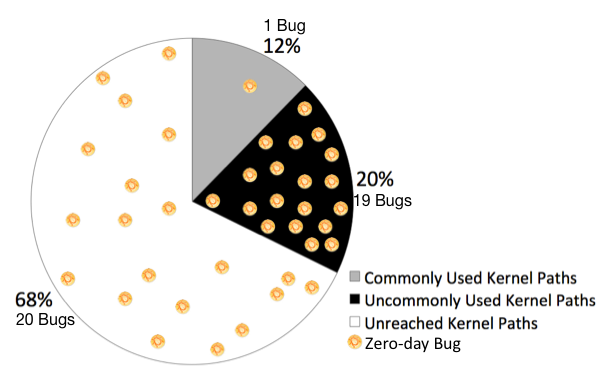
\includegraphics[width=1.0\columnwidth]{diagram/kernel_coverage.png}
\caption{\small Percentage of different kernel areas that were reached during
 LTP and Trinity system call fuzzing experiments, with the zero-day kernel bugs identified
 in each area.}
\label{fig:coverage}
\end{figure}

\section{Design Options for Secure Virtualization Systems}
\label{sec.design}

Providing essential system functionality without exposing privileged code is one of the
primary challenges. 
Currently, there are two basic approaches.
One, called ``System Call Interposition (SCI)," checks and passes system calls
through to the underlying kernel. The other, we call ``functionality
reimplementation," 
\yanyan{is this the official name?} 
\yiwen{No. We can come up with a better one.}
requires rebuilding system functionality with new code. In the
following, we show that both methods are limited in their ability to
prevent attacks in the kernel. 
With our metric in Section~\ref{sec.metric}, 
we propose a new design scheme named ``Lock-in-Pop" that combines safer reimplementation
within a secure environment, and accesses only popular code paths through a
very small trusted computer base.


\subsection{System Call Interposition (SCI)}
SCI is the long-standing idea behind sandboxing systems like Janus
\cite{Janus0:96, Janus:99}. It relies on the underlying kernel
to provide system functionality. To prevent attackers from undermining the system,
SCI uses a system call filter to mediate requests
from untrusted user code instead of allowing it to go directly to the kernel.
The filter checks a predefined security policy to decide which system calls are
allowed to pass to the underlying kernel, and which ones must be stopped.
Figure \ref{fig:design_system_call_interposition} illustrates the general design
of a system call interposition system. System administrators have direct access to 
setting and changing the security policies through a policy engine. 
This key part of the system would pose critical security threat if compromised, thus making it 
one component of the trusted computing base. 

\begin{figure}%[h]
\centering
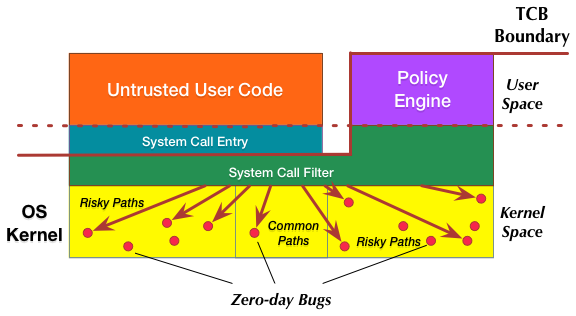
\includegraphics[width=1.0\columnwidth]{diagram/Virtualization_Design_Model_03.png}
\caption{\small Schematic of System Call Interposition.}
\label{fig:design_system_call_interposition}
\end{figure}  

SCI was once popular 
%approach to the design of secure virtualization systems because 
as it gave developers the ability to set and enforce security policies. 
%\lois{I think I asked this during the last revision. You say ``was"
%a popular approach. Is it not a popular approach anymore?}
%\yiwen{It is not a popular approach anymore, since no modern design could simply rely on 
%this idea to build practical system.}
However, this design
is limited by its overly complicated approach to policy decisions and implementation.
To make a policy decision, the system needs to
obtain and interpret the OS state (e.g., permissions, user groups, register flags) 
associated with the programs it is monitoring.
The complexity of OS states makes this process difficult and can lead to
inaccurate policy decisions.
Second, there are many indirect paths in the kernel that can be accessed.
Overlooking those paths by security policy makers would render the
system call interposition policy ineffective, as attackers are able to
bypass the imposed security checks. 
Moreover, many side-effects of blocking
certain system calls could affect the function of desired system calls.
It is difficult for developers to fully understand the side-effects of all the
system calls in an interface as complex as the UNIX API. 
For example, many applications that rely on \texttt{setuid} fail to check its return value. 
If \texttt{setuid} is blocked and fails, these applications will continue to function in a compromised state, 
with incorrect permissions and privileges. 
The above limitations make it very challenging to design and build a secure virtualization system using
system call interposition alone.

\subsection{Functionality Reimplementation}
Systems such as  Drawbridge \cite{Drawbridge-11},
 Bascule \cite{Bascule}, and Graphene \cite{Graphene-14} can
provide richer functionality and run complex programs than most systems built
with SCI. These systems have their own system
interfaces and libraries. Some virtualization
systems, such as OS VM systems VirtualBox, and VMWare Workstation, even have the
full functionalities of an OS reimplemented in their codebase. We call such a design
``functionality reimplementation."

\begin{figure}%[h]
\centering
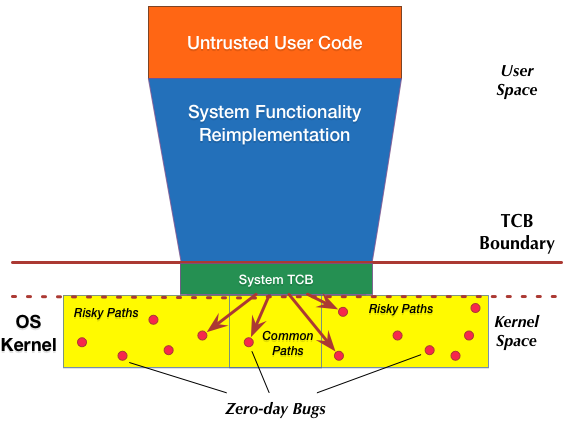
\includegraphics[width=1.0\columnwidth]{diagram/Virtualization_Design_Model_02.png}
\caption{\small Schematic of Functionality reimplementation System.}
\label{fig:design_functionality_reimplementation}
\end{figure}

The key of this design is to not fully rely on the underlying
kernel for system functions. Instead, critical OS functions are re-written with new
code. As illustrated in Figure \ref{fig:design_functionality_reimplementation}, 
this design reimplements its own system functionalities to provide to user code. 
When it has to %communicate with the kernel to
access resources like memory, CPU, and disk storage, the system accesses the kernel directly with
its underlying TCB code. 
%which can access the kernel directly.
For example, Graphene \cite{Graphene-14} reimplements
its own Linux system calls in 
\texttt{libLinux.so}. When it needs to acquire resources from
the kernel, it uses a
Platform Adaptation Layer (PAL)  that has access to the kernel
and provides basic ABI functions to the OS library.

Functionality reimplementation provides a more realistic solution to building
virtualization systems than earlier efforts, and offers rich functionality.
However, hundreds of vulnerabilities in existing virtualization systems have still been
reported over the past ten years~\cite{NVD}. One shortcoming of such systems is the size
of the implemented components. To provide rich functions, systems using this design have
introduced larger codebases and increased the size of their TCBs. In addition, the
complex semantics of OS functions can easily result in bugs and vulnerabilities in
reimplementation. Some vulnerabilities
can directly cause a privilege escalation, which allows attackers to escape the sandbox
and execute arbitrary code on the host OS. 
For example, a vulnerability in VMWare's codebase caused by buffer overflows in the VIX
API allowed local users to escape the guest VM and 
gain privilege to execute arbitrary code in the host
OS, even shellcode to access the kernel of the host OS~\cite{CVE-2008-2100}. 

Even operations that are considered
legal and harmless in the guest OS may open up risky system call paths in the underlying
host OS and cause a problem.
This type of problem can be fatal, 
as it can reach and trigger vulnerabilities in the underlying OS kernel.

\subsection{Lock-in-Pop: Staying on the Beaten Path }
A weakness of the previous approaches is the inevitable contact
between the privileged kernel code and the untrusted application. 
By leveraging our key observation 
that ``popular, frequently-used kernel paths contain fewer bugs" we propose a design
in which all code including the complex part
of the operating system interface should access only
popular kernel paths through a small TCB. As it ``locks" all functionality 
requests into only the ``popular" paths, we dubbed the
design ``Lock-in-Pop."

\begin{figure}%[h]
\centering
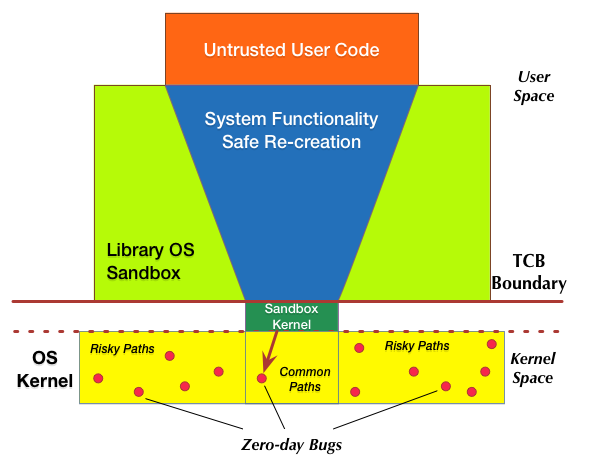
\includegraphics[width=.9\columnwidth]{diagram/Virtualization_Design_Model_01.png}
\caption{\small ``Lock-in-Pop''System ensures safe execution of untrusted user code
despite existing potential zero-day bugs in the OS kernel.}
\label{fig:design_safe_reimplementation}
\end{figure}

In addition, the system is entirely in the userspace, and both the size of 
the sandbox kernel and its access to the OS kernel is restricted
(Figure \ref{fig:design_safe_reimplementation}). Any complex or possibly risky system
functions that require contact with the OS kernel is re-created using
memory-safe code and is contained within a sandbox. This approach has advantages
over the others that require modifications to
the OS kernel (Section {\ref{sec.metric}). The isolation provided by placing
``Lock-in-Pop'' in the userspace is also an added protection over functionality
reimplemention. If a modified module in the OS kernel is compromised, it
exposes kernel privileges that could allow attacks 
in the underlying system and any applications in the userspace.

As shown in Figure \ref{fig:design_safe_reimplementation}, the key to  
``Lock-in-Pop'' is to construct a set of safe system functions within 
the library OS sandbox. 
The library OS sandbox responds to the system call requests and
returns results to the user code, if the requests are granted.
It is comprised of two parts: a sandbox kernel that provides access to basic but critical
system calls, and a system functionality safe reimplementation \yanyan{reconstruction?} that implements more
complex calls, such as symbolic link system call. 
The sandbox kernel forms the only TCB of our library OS, and is kept
extremely small and simple so that it is easy to verify its security.
The sandbox code provides an API that performs a few critical system calls with
the most basic parameters, such as writing data to the file system
and communicating with the network. 
%The kernel utilizes the most simplistic calls
%possible with the most basic arguments. 
The system functionality safe reimplementation 
is then built on top of the sandbox kernel. One important design rule is to only rely on the 
sandbox kernel API when trying to acquire hardware resources from the underlying OS kernel. 
The safe reimplementation will then use those basic resources, such as memory allocations, 
network sockets, and file descriptors to construct a virtual system interface, which will be 
provided to untrusted user code. 

%With the system functionality safe reimplementation, unmodified user code is able to run on top of our designed system.
It is important to note that our design does not rely on any specific technique or tool, and it is possible
to choose from several different techniques that fit specific security requirements.
The following section describes one implementation of our design called Lind.
\section{Implementation of Lind}
\label{sec.implementation}

Based on the design in Section \ref{sec.design},
we implemented a secure sandbox system, Lind,
for running untrusted user programs in vulnerable OS kernels.
Lind adopts two basic technologies as its building blocks\textendash
%Google's Native Client (NaCl), and Seattle's Repy.
%
%As described in Figure \ref{fig:design} and Section 4.2, our design has
%two main components\textendash a computation module that isolates the
%application and a library OS module that isolates the complex
%portions of POSIX, a standard OS interface Lind provides. We choose
Google's Native Client (NaCl)~\cite{NaCl-09} as the computation
module for efficient execution of legacy code in the
form of x86 and ARM binaries, and
Seattle's Repy~\cite{Repy-10} as the library OS.
%(Figure \ref{fig:architecture}), since it is a restricted subset of Python,
%that works as a sandbox to provide a safer environment to run untrusted code.

%\begin{figure}%[h]
%\centering
%	\includegraphics[width=1.0\columnwidth]{diagram/lind_architecture_new.png}
%	\caption{Architecture of Lind including various components such as NaCl, NaCl glibc, and Repy Sandbox.
%	User level applications will issue system calls that are dispatched through the Repy OS connector that bridges the Lind system to the OS Kernel.}
%\label{fig:architecture}
%\end{figure}

\textbf{Native Client.}
We use NaCl to isolate the computation of the user application
from the kernel. NaCl allows Lind to work on most types of legacy code.
It compiles the programs to produce a binary with software fault isolation.
This prevents the majority of the application from performing system calls
or executing arbitrary instructions.
%
To perform a system call, the application will call into a small privileged
part of the NaCl TCB that forwards system calls, usually to the OS for
processing. To build Lind, we changed the NaCl TCP to
forward these calls to our library OS that we call SafePOSIX (details below)
for processing.
% the following doesn't say anything new
%The NaCl glibc module contains stubs that reject operations
%that Chrome would not handle.  We added functionality to NaCl's glibc so that
%those calls could be forwarded into SafePOSIX for processing.

%NaCl can perform the functions required by the computation module well, and it is easy to
%connect with our system API module because NaCl uses glibc to perform system calls.
%Modification to NaCl's glibc would allow us to redirect those system call requests to our own system API module.
%
%NaCl is a sandbox used to execute untrusted x86 native code.
%It aims to give applications the computational performance of native applications without compromising safety.
%NaCl uses software fault isolation and a secure runtime to direct system interaction and
%side effects through interfaces managed by the program. It provides operating system portability
%for binary code while supporting performance-oriented features, such as thread support,
%instruction set extensions, such as SSE, and use of compiler intrinsics and a hand-coded assembler.
%It also allows the efficient execution of legacy code in the form of x86 and ARM binaries
%that are built with a lightly modified compiler tool chain.

\textbf{Seattle's Repy.}
To build an API to access the safe parts of the underlying kernel, we need
two things.  First, we need a restricted sandbox that isolates computation
and only allows access to commonly used kernel paths.  We used
Seattle's Repy~\cite{Repy-10} sandbox to perform this task.
Second, we need to build a POSIX implementation to run within that sandbox.

%pplications. For Lind, we used Repy to build our system API module.
%To be more specific, our system API module has a very small sandbox kernel
%as TCB,  written with Python. On top of the sandbox kernel,
%we use Repy code to safely reimplement complex system functions.

\textit{The Repy Sandbox Kernel.}
A natural concern with any sandbox design is that bugs will simply be pushed into
another part of the trusted code base.  As it is the only piece of code added
to the system call paths of the TCB, the sandbox kernel's security is of
paramount concern.
%The sandbox kernel needs to be secure and bug-free.
%Because it is the TCB of the system, any bugs in it could cause fatal problems.
%and allow attackers to access the OS kernel and gain kernel privilege.
We used Seattle's Repy system API due to its tiny sandbox kernel
(comprised of around 8K LOC), and its ability to provide straightforward
access to the minimal set of the system call API needed to build general
computational functionality. Repy allows
%fit our key design principle that our proposed system should
access only to the safe portions of the OS kernel with 33 basic API
functions, including 13 network functions, 6 file functions, 6 threading functions,
and 8 miscellaneous functions~\cite{Repy-10, RepyKernel}. The code is
written using style guidelines designed to ease security auditing
 of the code~\cite{style}. Most of these functions are simple and
regularly used system calls that access the commonly used kernel paths.

%\begin{table}
%\centering
%\caption {Repy sandbox kernel capabilities that supports NaCl functions, such as networking, file I/O operations and threading.}
%
%  \begin{tabular}{ | p{2.5cm} | p{4.5cm} |}
%  \hline
%  \textbf{Repy Function} & \textbf{Available System Calls}  \\ \hline
%
%Networking & \emph{gethostbyname, openconnection, getmyip, socket.send, socket.receive, socket.close,
%listenforconnection, tcpserversocket.getconnection, tcpserversocket.close, sendmessage, listenformessage,
%udpserversocket.getmessage, and udpserversocket.close.} \\ \hline
%
%I/O Operations & \emph{openfile, file.close, file.readat, file.writeat, listfiles, and removefile.} \\ \hline
%
%Threading & \emph{createlock, sleep, lock.acquire, lock.release, createthread, and getthreadname.} \\ \hline
%
%Miscellaneous Functions & \emph{getruntime, randombytes, log, exitall, createvirtualnamespace,
%virtualnamespace.evaluate, getresources, and getlasterror.}  \\ \hline
%    \end{tabular}
%    \label{table:RepyKernel}
%\end{table}

%\begin{table}
%\centering
%\scriptsize
%\caption {System Functions in the Repy Sandbox Kernel.  \cappos{Need to
%clearly explain the takeaway.}}
%\begin{tabular}{|l|}
%  \hline
% \textbf{Network Functions} \\
%  \hline
%  gethostbyname(name) \\
%  \hline
%  getmyip() \\
%  \hline
%  openconnection(destip, destport, localip, localport, timeout) \\
%  \hline
%  socket.close() \\
%  \hline
%  socket.recv(numbytes) \\
%  \hline
%  socket.send(message) \\
%  \hline
%  listenforconnection(localip, localport) \\
%  \hline
%  tcpserversocket.getconnection() \\
%  \hline
%  tcpserversocket.close()\\
%  \hline
%  sendmessage(destip, destport, message, localip, localport) \\
%  \hline
%  listenformessage(localip, localport) \\
%  \hline
%  udpserversocket.getmessage() \\
%  \hline
%  udpserversocket.close() \\
%  \hline \hline
%  \textbf{File Functions} \\
%  \hline
%  openfile(filename, create) \\
%  \hline
%  file.close() \\
%  \hline
%  file.readat(sizelimit, offset) \\
%  \hline
% file.writeat(data, offset) \\
%  \hline
%  listfiles() \\
%  \hline
%  removefile(filename) \\
%  \hline \hline
%  \textbf{Threading Functions} \\
%  \hline
%  createlock() \\
%  \hline
%  lock.acquire(blocking) \\
%  \hline
%  lock.release() \\
%  \hline
%  createthread(function) \\
 % \hline
 % sleep(seconds) \\
  %\hline
  %getthreadname() \\
  %\hline \hline
  %\textbf{Miscellaneous Functions} \\
  %\hline
 % getruntime() \\
  %\hline
 % randombytes() \\
  %\hline
  %log(*args) \\
  %\hline
  %exitall() \\
  %\hline
  %createvirtualnamespace(code, name) \\
  %\hline
  %virtualnamespace.evaluate(context) \\
  %\hline
  %getresources() \\
  %\hline
  %getlasterror() \\
  %\hline
%\end{tabular}
%\label{table:RepyKernel}
%\end{table}


The Repy kernel code has been
audited by a professional penetration tester.  Since 2010, there has also been
a bug bounty program for security flaws in the sandbox.
The code is deployed in daily use across thousands of devices,
including on the Seattle testbed \cite{seattle}, and has been examined by
hundreds of parties.
%Developers have reported
%XXX issues for problems in other parts of the systems. However,
To date no security flaws have been found in the sandbox kernel.
%This does not provide any strong guarantees that bugs do not exist, and if
%they do, the security of the system could be compromised.
%However,
Having a small, easily auditable piece of code thus helps to reduce the
risk of such occurrence.

\textit{The SafePOSIX Reimplementation.}
The key responsibility of our system API module is to serve system call requests from user code.
In Lind, those system call requests are issued from the user code,
received by NaCl, and then redirected to our system API module.
The API module includes a POSIX API to serve those requests.

A POSIX API is a set of standard operating system interfaces that provide operating system functions
to the user code. However, the POSIX API is large and complex enough that it is
very hard to ensure that its implementation is secure and bug-free.
%
%Our choice to use Repy helped us solve this architectural security problem.
Since Repy is a programming language sandbox, it can provide the ideal isolation
needed to construct our POSIX API. In Lind,
complex system functions are reimplemented using Repy code,
based on the ``safe-reimplement'' principle from our design in Section~{\ref{sec.design}}.

\textbf{Dual-Sandbox Design.}
The kernel interface is extremely rich and hard to protect.
In order to have minimal impact on the kernel, as well as provide sufficient API for legacy applications,
we need to have one sandbox focusing on protecting the kernel and providing POSIX API.
Lind combines the NaCl and Repy sandboxing techniques to provide native computation and
safe access to the system.
%Untrusted programs are run in NaCl,
%but access to all system resources is diverted to a Repy program.\yanyan{SafePOSIX?}
%This program is responsible for accessing the system on behalf of the Lind library
% OS. A NaCl sandbox is built on top of the Repy sandbox.
%
To service a system call in NaCl, a server routine in Lind marshals its arguments into a text string,
and sends the call and the arguments to the Repy sandbox.
The library OS then executes the appropriate system call, marshals the result and
returns it back to NaCl. Eventually, the result is returned as the appropriate native type to the calling program.

%Lind is designed to minimize the need to modify either sandbox. This is possible
%because the TCB of both were extremely small, and because the Lind code is run
%in both.
%\lois{Another odd sentence Yiwen and I discussed. I thought I knew how to
%fix it, but it still does not make sense. I would delete it.}

%The only complex part of Lind is the library OS, which runs in Repy.
%However, because Python is a very powerful language that provides rich functions,
%it helps to make the construction of Lind easier. The downside of Python is that
%some consider the language ``slow'',
%because it is dynamically typed rather than statically typed, it is interpreted rather than compiled,
%and Python's object model can lead to inefficient memory access.
%Nevertheless, the internals of an application in Lind are run in NaCl, a very high performance
%environment.

%This balances the performance of the system, with the ease of implementation and maintenance of the library OS component of Lind.
%\yanyan{I think this paragraph can be cut.}

%Lind is portable.
%Programs running inside Lind are using a standard POSIX glibc interface,
%and, since the Lind runtime is strictly user-level, it can work on many different platforms
%including Linux, Mac OS X and Windows.
Our design could include more than two sandboxes, e.g., by sandboxing the sandbox
kernel. However, in a secure system,
the lowest level sandbox eventually must have some fundamental,
even if limited, access to system resources, such as memory, and storage, threads.
Even if we were to sandbox the sandbox kernel and have additional sandboxes,
the one at the bottom level will still access the OS kernel in a similar way.
Thus, having multiple sandboxes does not provide any extra security benefits.

The lightweight and minimized overhead is another feature of the dual-sandbox design. Because the sandbox only
 incurs overhead when there is a system call, overall overhead for Lind is low.
 Yet, it does not sacrifice performance for cost.
Lind uses a native interface for execution,
allowing CPU-and-memory-intensive applications to run at speeds that are equivalent
 to NaCl and near native speed.
\section{Evaluation}
\label{sec.evaluation}

%In order to evaluate Lind's effectiveness in providing kernel protection, we
%conducted a series of experiments designed to answer four fundamental questions:

In order to evaluate Lind's effectiveness in containing untrusted code and
protecting OS kernel, we conducted a series of experiments to answer
four fundamental questions:

\textit{How does Lind compare to other virtualization systems
in protecting against zero-day Linux kernel bugs?}
(Section~{\ref{Linux-Kernel-Bug-Test-and-Evaluation}})
%\yiwen{I am wondering if we should say ``zero-day bugs'' instead of ``historical bugs''.}

\textit{How much of the underlying kernel code is exposed, and is thus
vulnerable in different virtualization systems?}
(Section~{{\ref{Reachable-Kernel-Trace-Analysis-for-Different-Virtualization-Systems}})
%\yiwen{This question may need to be refined. Why is the question important to the readers?
%What is the take-away? The reachable kernel paths reflect an important security property
%of the system design. We want to express this point.}
%\lois{I made an attempt
%here at addressing your concerns. I agree its an important point to emphasize correctly.
%We might need to tweak it a bit more.}

\textit{If Lind's SafePOSIX reimplementation has bugs, how much of a threat does this pose?}
(Section~{{\ref{Reachable-Kernel-Trace-Analysis-for-Repy-Sandbox}})

\textit{In the Lind prototype, what is the expected overhead in
real-world applications?}
(Section~{{\ref{Performance-Evaluation}})

This section describes the setup of our experiments, 
and shows our experiment results. 
%and argues how the results support the merits of our secure design and its Lind prototype.
%\yiwen{If we claim the above sentence, then we need to say more about our secure design,
%which can be hard. Possibly remove ``our secure design'' and just keep ``Lind
%prototype.''}
%\lois{There might be some value to keeping the phrase in, since we
%are emphasizing the design and not the product.}
%
%\subsection{Experiment Methodology}
%
Our evaluation strategy was to directly compare the performance of Lind
against
seven other existing virtualization systems\textendash VirtualBox, VMWare
Workstation,
Docker, LXC, QEMU, KVM and Graphene. 
We chose those seven systems because they are widely used virtualization systems 
that are representative of the most popular design models. Among them, 
VirtualBox and VMWare Workstation are very popular commercial OS VM products. 
LXC and KVM are Linux kernel modules, Docker and QEMU are well known open source projects. 
And Graphene is an open source research project. 
We also compared against Native Linux as a baseline for comparison. 
%Because Native Linux is the original OS,
%without virtualization and additional protection, this data helps to
%clarify the security benefits of Lind,
%as well as whatever performance overhead costs the system may incur.


%\subsection{Experimental Setup, Results and Analysis}

%As dictated by the study questions listed above, our tests were conducted
%and appraised primarily from a security perspective
%(Section~{{\ref{Linux-Kernel-Bug-Test-and-Evaluation}} --
%%\S{\ref{Reachable-Kernel-Trace-Analysis-for-Different-Virtualization-Systems}},
%Section~{{\ref{Reachable-Kernel-Trace-Analysis-for-Repy-Sandbox}}).
%However, to get some idea of its potential efficacy
%in real-world settings, we also measured and evaluated the performance
%overhead of Lind
%(Section~{{\ref{Performance-Evaluation}})

\subsection{Linux Kernel Bug Test and Evaluation}
\label{Linux-Kernel-Bug-Test-and-Evaluation}

\textbf{Setup.}
To evaluate how well each virtualization system protect the Linux kernel against 
reported zero-day bugs, we identified and examined a list of  69 historical bugs that have
specifically targeted Linux kernel 3.14.1 \cite{CVE-Datasource}. 
By analyzing security kernel patches for those bugs,
we identified the lines of code in the kernel that correspond to each one. 

In order to test if a bug can be triggered, we created or located C
code capable of exploiting each of the kernel bugs \cite{Exploit-Database}.
We were only able to trigger and obtain results for 35 out of the 69 bugs in our experiments, 
either because of a difficulty in clearly determining if triggering had occurred, or an inability,
at this time, to find code to trigger them. We decided to focus our study on
only these bugs and leave the other, more complex ones, to future work and analysis.

We compiled and ran the exploit C code under each virtualization system to
obtain their kernel traces, and then used our kernel trace safety metric to
determine if a specific bug was triggered.

%\lois{I think this whole first paragraph can come out. All this information has
%been stated already. This is an evaluation of the RESULTS}
%We attempted to
%trigger 35 identified Linux kernel bugs by running programs in
%Native Linux, VirtualBox, VMWare Workstation, Docker, Graphene,
%and Lind.
%The kernel bugs examined are capable of causing serious security problems.
%For example,the CVE-2014-8989 bug allows local users to bypass intended file
%permissions by leveraging a POSIX ACL.
%The potential risk of triggering these and other types of
%kernel bugs when running applications, is a problem that
%needs to be taken seriously.

\noindent
\textbf{Results.}
We found that a substantial number of bugs could be triggered in existing
virtualization systems, as shown in Table \ref{table:trigger_vulnerabilities}.
A full 35 out of 35 (100\%) bugs were triggered in Native Linux,
while the other programs had lower rates: 14/35 (40\%) in
VirtualBox,
11/35 (31.4\%)  in VMWare Workstation, 8/35 (22.9\%)  in Docker,
12/35 (34.3\%)  in LXC, 5/35 (14.3\%)  in QEMU, 5/35 (14.3\%)  in KVM,
and 8/35 (22.9\%) bugs in Graphene.
In comparison, only 1 out of 35 bugs  (2.9\%) was triggered in Lind.

To better understand these results, 
%and particularly why Lind's performance was so strong, 
we take a closer look at four
vulnerabilities from Table \ref{table:trigger_vulnerabilities}. These short case
studies show how different system design philosophies can have 
different security impacts.
%\yiwen{The following analysis needs to be refined. 
%I need to rework with more information about the system call paths.}

\begin{table*}[!ht]
\scriptsize
\centering

\caption {\small Linux Kernel Bugs, and Vulnerabilities in Different Virtualization Systems
({\color{red}\ding{51}}: vulnerability triggered;
{\color{blue}\ding{51}}: vulnerability triggered with Guest Additions; \ding{55}: vulnerability
not triggered).}

%\resizebox{0.68\textwidth}{!}{\begin{minipage}{\textwidth}

\begin{tabular}{|p{1.7cm}|l|l|p{1cm}|p{1cm}|p{.8cm}|p{1cm}|p{.8cm}|p{1cm}|p{.8cm}|}\hline

\multirow{2}{1.7cm}{\bf Vulnerability}    &  \multirow{2}{.7cm}{\bf Native Linux}  &  \multirow{2}{*}{\bf VirtualBox}
&  \multirow{2}{.7cm}{\bf VMWare}
 & \multirow{2}{1cm}{\bf Docker} & \multirow{2}{1cm}{\bf LXC} &
\multirow{2}{1cm}{\bf QEMU} & \multirow{2}{1cm}{\bf KVM} &
\multirow{2}{1cm}{\bf Graphene} & \multirow{2}{1cm}{\bf Lind} \\ 
& & & & & & & & & \\
\hline

 CVE-2015-5706 & \multirow{1}{.7cm}{{\color{red}\ding{51}}} & {\color{blue}\ding{51}} &
\multirow{1}{1cm}{{\color{blue}\ding{51}}} & \multirow{1}{1cm}{{\color{red}\ding{51}}} & 
\multirow{1}{1cm}{{\color{red}\ding{51}}} & \multirow{1}{1cm}{{\color{red}\ding{51}}} & 
\multirow{1}{1cm}{{\color{red}\ding{51}}} & \multirow{1}{1cm}{{\color{red}\ding{51}}} & 
\ding{55}  \\

 CVE-2015-0239 & \multirow{1}{.7cm}{{\color{red}\ding{51}}} & {\color{red}\ding{51}} &
\multirow{1}{1cm}{{\color{red}\ding{51}}} & \ding{55} & \multirow{1}{1cm}{{\color{red}\ding{51}}} &
\multirow{1}{1cm}{{\color{red}\ding{51}}} & \multirow{1}{1cm}{{\color{red}\ding{51}}} &
 \ding{55}  & \ding{55}  \\
 
 CVE-2014-9584 & \multirow{1}{.7cm}{{\color{red}\ding{51}}} & \ding{55}  &
 \ding{55}  & \ding{55} & \ding{55} &
 \ding{55}& \ding{55} &
 \ding{55}  & \ding{55}  \\
 
 CVE-2014-9529 & \multirow{1}{.7cm}{{\color{red}\ding{51}}} & {\color{red}\ding{51}}  &
\ding{55}  & \ding{55} & \multirow{1}{1cm}{{\color{red}\ding{51}}} &
\ding{55}& \ding{55} &
\ding{55}  & \ding{55}  \\

 CVE-2014-9322 & \multirow{1}{.7cm}{{\color{red}\ding{51}}} & {\color{red}\ding{51}}  &
\ding{55}  & \multirow{1}{1cm}{{\color{red}\ding{51}}} & \multirow{1}{1cm}{{\color{red}\ding{51}}} &
\multirow{1}{1cm}{{\color{red}\ding{51}}} & \multirow{1}{1cm}{{\color{red}\ding{51}}} &
\multirow{1}{1cm}{{\color{red}\ding{51}}}  & \ding{55}
\\

 CVE-2014-9090 & \multirow{1}{.7cm}{{\color{red}\ding{51}}} & \ding{55}  &
 \ding{55}  & \ding{55} & \ding{55} &
 \ding{55} & \ding{55} &
 \ding{55}  & \ding{55}  \\
 
 CVE-2014-8989 & \multirow{1}{.7cm}{{\color{red}\ding{51}}} & {\color{red}\ding{51}} &
\multirow{1}{1cm}{{\color{red}\ding{51}}} & \multirow{1}{1cm}{{\color{red}\ding{51}}} & 
\multirow{1}{1cm}{{\color{red}\ding{51}}} & \multirow{1}{1cm}{{\color{red}\ding{51}}} & 
\multirow{1}{1cm}{{\color{red}\ding{51}}} & \multirow{1}{1cm}{{\color{red}\ding{51}}} & 
\ding{55}  \\

 CVE-2014-8559 & \multirow{1}{.7cm}{{\color{red}\ding{51}}} & \ding{55}  &
 \ding{55}  & \ding{55} & \ding{55} &
 \ding{55} & \ding{55} &
 \ding{55}  & \ding{55}  \\
 
 CVE-2014-8369 & \multirow{1}{.7cm}{{\color{red}\ding{51}}} & \ding{55}  &
 \ding{55}  & \ding{55} & \ding{55} &
 \ding{55} & \ding{55} &
 \ding{55}  & \ding{55}  \\
 
 CVE-2014-8160 & \multirow{1}{.7cm}{{\color{red}\ding{51}}} & {\color{red}\ding{51}} &
\multirow{1}{1cm}{{\color{red}\ding{51}}} & \ding{55} & \multirow{1}{1cm}{{\color{red}\ding{51}}} &
\ding{55} & \ding{55} &
\ding{55}  & \ding{55}  \\

 CVE-2014-8134 & \multirow{1}{.7cm}{{\color{red}\ding{51}}} & {\color{red}\ding{51}} &
\multirow{1}{1cm}{{\color{red}\ding{51}}} & \ding{55} & \multirow{1}{1cm}{{\color{red}\ding{51}}} &
\ding{55} & \ding{55} & \multirow{1}{1cm}{{\color{red}\ding{51}}}  & \ding{55}
\\

 CVE-2014-8133 & \multirow{1}{.7cm}{{\color{red}\ding{51}}} & {\color{red}\ding{51}}  &
\ding{55}  & \ding{55} & \ding{55} &
\ding{55} & \ding{55} &
\ding{55}  & \ding{55}  \\

 CVE-2014-8086 & \multirow{1}{.7cm}{{\color{red}\ding{51}}} & {\color{blue}\ding{51}} &
\multirow{1}{1cm}{{\color{blue}\ding{51}}} & \multirow{1}{1cm}{{\color{red}\ding{51}}} & 
\multirow{1}{1cm}{{\color{red}\ding{51}}} &
\ding{55} & \ding{55} &
\ding{55} & \ding{55}  \\

 CVE-2014-7975 & \multirow{1}{.7cm}{{\color{red}\ding{51}}} & \ding{55}  &
 \ding{55}  & \ding{55} & \ding{55} &
 \ding{55} & \ding{55} &
 \ding{55}  & \ding{55}  \\
 
 CVE-2014-7970 & \multirow{1}{.7cm}{{\color{red}\ding{51}}} & \ding{55}  &
 \ding{55}  & \ding{55} & \ding{55} &
 \ding{55} & \ding{55} &
 \ding{55}  & \ding{55}  \\
 
 CVE-2014-7842 & \multirow{1}{.7cm}{{\color{red}\ding{51}}} & \ding{55}  &
 \ding{55}  & \ding{55} & \ding{55} &
 \ding{55} & \ding{55} &
 \ding{55}  & \ding{55}  \\
 
 CVE-2014-7826 & \multirow{1}{.7cm}{{\color{red}\ding{51}}} & {\color{red}\ding{51}} &
\multirow{1}{1cm}{{\color{red}\ding{51}}} & \ding{55} & \ding{55}  &
\ding{55} & \ding{55} & \multirow{1}{1cm}{{\color{red}\ding{51}}}  & \ding{55}
\\

 CVE-2014-7825 & \multirow{1}{.7cm}{{\color{red}\ding{51}}} & {\color{red}\ding{51}} &
\multirow{1}{1cm}{{\color{red}\ding{51}}} & \ding{55} & \ding{55} &
\ding{55} & \ding{55} & \multirow{1}{1cm}{{\color{red}\ding{51}}}  & \ding{55}
\\

 CVE-2014-7283 & \multirow{1}{.7cm}{{\color{red}\ding{51}}} & \ding{55}  &
 \ding{55}  & \ding{55} & \ding{55} &
 \ding{55} & \ding{55} &
 \ding{55}  & \ding{55}  \\
 
 CVE-2014-5207 & \multirow{1}{.7cm}{{\color{red}\ding{51}}} & \ding{55}  &
 \ding{55}  & \ding{55} & \ding{55} &
 \ding{55} & \ding{55} &
 \ding{55}  & \ding{55}  \\
 
 CVE-2014-5206 & \multirow{1}{.7cm}{{\color{red}\ding{51}}} & \ding{55}  &
\multirow{1}{1cm}{{\color{red}\ding{51}}}  & \multirow{1}{1cm}{{\color{red}\ding{51}}} & 
\multirow{1}{1cm}{{\color{red}\ding{51}}} &
\ding{55} & \ding{55} &
\ding{55}  & \ding{55}
\\

 CVE-2014-5045 & \multirow{1}{.7cm}{{\color{red}\ding{51}}} & \ding{55}  &
 \ding{55}  & \ding{55} & \ding{55} &
 \ding{55} & \ding{55} &
 \ding{55}  & \ding{55}  \\
 
 CVE-2014-4943 & \multirow{1}{.7cm}{{\color{red}\ding{51}}} & \ding{55}  &
 \ding{55}  & \ding{55} & \ding{55} &
 \ding{55} & \ding{55} &
 \ding{55}  & \ding{55}  \\
 
 CVE-2014-4667 & \multirow{1}{.7cm}{{\color{red}\ding{51}}} & \ding{55}  &
 \ding{55}  & \ding{55} & \ding{55} &
 \ding{55} & \ding{55} & \multirow{1}{1cm}{{\color{red}\ding{51}}}  & \ding{55}  \\
 
 CVE-2014-4508 & \multirow{1}{.7cm}{{\color{red}\ding{51}}} & \ding{55}  &
 \ding{55}  & \ding{55} & \ding{55} &
 \ding{55} & \ding{55} &
 \ding{55}  & \ding{55}  \\
 
 CVE-2014-4171 & \multirow{1}{.7cm}{{\color{red}\ding{51}}} & {\color{red}\ding{51}} &
\multirow{1}{1cm}{{\color{red}\ding{51}}} & \multirow{1}{1cm}{{\color{red}\ding{51}}} & 
\multirow{1}{1cm}{{\color{red}\ding{51}}} & \multirow{1}{1cm}{{\color{red}\ding{51}}} & 
\multirow{1}{1cm}{{\color{red}\ding{51}}} & \multirow{1}{1cm}{{\color{red}\ding{51}}} & 
\multirow{1}{1cm}{{\color{red}\ding{51}}}  \\

 CVE-2014-4157 & \multirow{1}{.7cm}{{\color{red}\ding{51}}} & \ding{55}  &
 \ding{55}  & \ding{55} & \ding{55} &
 \ding{55} & \ding{55} &
 \ding{55}  & \ding{55}  \\
 
 CVE-2014-4014 & \multirow{1}{.7cm}{{\color{red}\ding{51}}} & \ding{55}  &
\multirow{1}{1cm}{{\color{red}\ding{51}}}  & \multirow{1}{1cm}{{\color{red}\ding{51}}} & 
\multirow{1}{1cm}{{\color{red}\ding{51}}} &
\ding{55} & \ding{55} &
\ding{55}  & \ding{55}
\\

 CVE-2014-3940 & \multirow{1}{.7cm}{{\color{red}\ding{51}}} & {\color{blue}\ding{51}}  &
\ding{55}  & \multirow{1}{1cm}{{\color{red}\ding{51}}} & \multirow{1}{1cm}{{\color{red}\ding{51}}} &
\ding{55} & \ding{55} &
\ding{55}  & \ding{55}  \\

 CVE-2014-3917 & \multirow{1}{.7cm}{{\color{red}\ding{51}}} & {\color{red}\ding{51}}  &
\ding{55}  & \ding{55} & \ding{55} &
\ding{55} & \ding{55} &
\ding{55}  & \ding{55}  \\

 CVE-2014-3153 & \multirow{1}{.7cm}{{\color{red}\ding{51}}} & \ding{55}  &
  \ding{55}  & \ding{55} & \ding{55} &
  \ding{55} & \ding{55} &
  \ding{55}  & \ding{55}  \\
  
 CVE-2014-3144 & \multirow{1}{.7cm}{{\color{red}\ding{51}}} & \ding{55}  &
 \ding{55}  & \ding{55} & \ding{55} &
 \ding{55} & \ding{55} &
 \ding{55}  & \ding{55}  \\
 
 CVE-2014-3122 & \multirow{1}{.7cm}{{\color{red}\ding{51}}} & \ding{55}  &
 \ding{55}  & \ding{55} & \ding{55} &
 \ding{55} & \ding{55} &
 \ding{55}  & \ding{55}  \\
 
 CVE-2014-2851 & \multirow{1}{.7cm}{{\color{red}\ding{51}}} & \ding{55}  &
 \ding{55}  & \ding{55} & \ding{55} &
 \ding{55} & \ding{55} &
 \ding{55}  & \ding{55}  \\
 
 CVE-2014-0206 & \multirow{1}{.7cm}{{\color{red}\ding{51}}} & \ding{55}  &
 \ding{55}  & \ding{55} & \ding{55} &
 \ding{55} & \ding{55} &  \ding{55}  & \ding{55}  \\
\hline

 {\bf Vulnerabilities Triggered} & \multirow{2}{1cm}{\bf 35/35 (100\%)} & {\bf 14/35 (40.0\%)} &
 {\bf 11/35 (31.4\%)}  & {\bf 8/35 (22.9\%)} & {\bf 12/35 (34.3\%)} & {\bf 5/35 (14.3\%)} & {\bf 5/35 (14.3\%)} &
 {\bf 8/35 (22.9\%)}  & {\bf 1/35 (2.9\%)}  \\
\hline
\end{tabular}
\label{table:trigger_vulnerabilities}
\end{table*}


\emph{\textbf{All systems vulnerable.}}  Representative bug: CVE-2014-4171.
This is the only vulnerability in our test that was triggered in every
system, including Lind. It resides inside the \texttt{mm/shmem.c} kernel path and
can be triggered by using \texttt{mmap()} system call to access a hole in the memory.
The \texttt{mmap()} call then invokes \texttt{shmem\_fault()}, which will cause contention
on \texttt{i\_mmap\_mutex}, and lead to a serious starvation of memory resource.
The reason that Lind triggered this bug is because \texttt{mmap()} cannot easily
be safely reimplemented inside our SafePOSIX API. The call sets up a
memory region where the OS will later
intervene and automatically convert all accesses into ones that reach the
underlying file.  The code does not explicitly make system calls, and as
a result, with Lind's design we cannot intercept those accesses and call through
the Repy sandbox kernel. Thus,
Lind allows \texttt{mmap()} calls to directly access the kernel, which
opens the chance to trigger this vulnerability. 
In the library OS system Graphene, similar to Lind, it does not reimplement the 
\texttt{mmap()} system call in its library module \texttt{libLinux}. Instead, when doing 
memory allocation operations like \texttt{malloc()} and \texttt{brk()}, Graphene will 
pass down those system calls to the underlying kernel, and rely on the kernel to 
perform the \texttt{mmap()} system function. 
KVM and LXC both reside inside the Linux kernel and inherit the \texttt{mmap()} system function 
from the kernel. QEMU is built on KVM, and relies on the KVM module to perform \texttt{mmap()} 
function. Docker is built on LXC, which relies on the LXC module to perform \texttt{mmap()} 
function. In VirtualBox and VMWare Workstation, the OS VM has its own mechanism to 
do memory management. During the initial setup, the OS VM needs to request memory resource 
by making \texttt{mmap()} to the host kernel. In addition, during the runtime of the VM process, 
when there is excessive memory usage, or reconfiguration of memory allocation, the VM kernel module 
will attempt to call \texttt{mmap()} to the host kernel. Thus, this vulnerability related with \texttt{mmap()} 
is exploitable under the virtualization systems that we tested. 

\emph{\textbf{Only Native Linux vulnerable.}}  Representative bug: CVE-2014-5045.
This vulnerability was only triggered inside Native Linux. It resides in the
\texttt{fs/namei.c} kernel path and was triggered because
the \texttt{mountpoint\_last()}
%\texttt{mountpoint\_last(struct nameidata *nd, struct path *path)}
function does not properly
maintain a reference count during attempts to use the \texttt{umount()} system call,
in conjunction with a symbolic link. Unmounting from a symbolic link could block 
another unmount operation, and allow attackers to cause a denial of service or 
deploy use-after-free exploitation. Lind does not implement symbolic link, but 
even similar functionality that might be risky is implemented entirely
within its SafePOSIX module. The bug would (at most) enable an attacker to execute
code within the Repy sandbox and would not harm other parts of the system. 
Graphene does not implement symbolic link in its Linux system call API, and thus avoids 
this problem. 
OS VM like VirtualBox and VMWare Workstation have their own metadata to maintain their file
directories and symbolic links, which do not directly rely on the host OS. 
%\cappos{Why did the flag in the first example
%work then?  Also, why doesn't this exist in Docker / LXC?}
Furthermore, symbolic links in those systems will be contained within the virtualization system's image,
and will not be able to reach the underlying host OS. In this case, those virtualization systems provide enough
isolation to prevent this bug.
Docker/LXC and QEMU/KVM happen to avoid this bug because their kernel module modified the Linux kernel 
that fixed this problem. It should be noted though that by their design model, they both tend to suffer from 
the same vulnerabilities that exist inside the Native Linux kernel. 

\emph{\textbf{Some systems safe, some systems vulnerable.}}  Representative bug: CVE-2014-8086.
This vulnerability was not triggered inside Graphene and Lind, but was triggered inside
VirtualBox, VMWare workstation, Docker, and Native Linux. It resides in
the \texttt{fs/ext4/file.c} kernel path, and can be triggered by a file system write
function call, made together with \texttt{fcntl} function call
with argument \texttt{F\_SETFL}, and \texttt{O\_DIRECT} flag. If triggered, it could
allow attackers to cause a denial of service (file unavailability). Both Lind and
Graphene prevented this bug, but for different reasons. Lind
implements \texttt{fcntl} in SafePOSIX, so the underlying kernel is not called.
Graphene checks and blocks certain system calls, including
a \texttt{fcntl} system call with the \texttt{O\_DIRECT} flag.
Other systems like VirtualBox, VMWare Workstation, Docker, and Native Linux,
all suffer from this vulnerability because calls go directly into the host OS
kernel.

\emph{\textbf{Only Lind safe.}}  Representative bug: CVE-2015-5706. As
shown in our results, this vulnerability was triggered in every
virtualization system we tested, except Lind. This vulnerability
is closely related to file system calls and file flags, resides in the \texttt{fs/namei.c}
kernel path, and can be triggered by making a \texttt{path\_openat()} function
call with file flag \texttt{O\_TMPFILE}. \texttt{path\_openat()} will jump to the wrong
place after \texttt{do\_tmpfile()}, and do \texttt{path\_cleanup()} twice. This would
allow local users to perform use-after-free exploitation to cause a denial of service.
This bug was not triggered in Lind, because it does not support the use of the
\texttt{O\_TMPFILE} file flag. In fact, the only call in the Repy sandbox that
opens a file does not take an argument for flags or other operations.  The
only arguments it takes are a filename (that must consist of a small number
of highly restricted characters) and a flag to indicate whether a file should
be created if one does not exist.
Other virtualization systems allow more complex configuration of flags to
pass through to the underlying OS kernel.
%\cappos{Why does VirtualBox pass this
%through?  My VirtualBox file system is a single VDI file.  How does this end
%up calling into the host OS's kernel and why?}  \cappos{Does this vary
%if you use a different FS type on VirtualBox?}
In this case, the \texttt{O\_TMPFILE} file flag was
allowed in Native Linux, VirtualBox, VMWare Workstation, Docker, and Graphene.


As shown in the above four cases, bugs are usually triggered by
complex system calls,
or basic system calls with complicated or rarely used flags.
The safely-reimplement design behind Lind, which controls access to the kernel and
minimizes exposure of vulnerable code, poses
the least risk of triggering bugs in the underlying OS kernel. 

%To better understand the connection between kernel access and the 
%triggering of vulnerable code, our next step is to 
We next look at the extent and type of exposure inherent in different
virtual security systems.

\subsection{Comparison of Kernel Code Exposure in Different Virtualization
Systems}
\label{Reachable-Kernel-Trace-Analysis-for-Different-Virtualization-Systems}

\begin{table}
\centering
\scriptsize
\caption{\small Reachable kernel trace analysis for different virtualization
systems.}
\begin{tabular}{|l|l|l|l|}
  \hline
  \multirow{3}{1.5cm}{\bf Virtualization system} & \multicolumn{3}{c|}{\bf Kernel trace} \\ \cline{2-4}
  & \multirow{2}{1.5cm}{Compared to native Linux} & \multirow{2}{1.5cm}{In common paths} & \multirow{2}{1cm}{In risky paths} \\
  & & & \\  \hline
  VirtualBox & 78.8 \% & 46.5 \% & 53.5 \% \\
  \hline
  \multirow{2}{1.5cm}{VMWare Workstation} & \multirow{2}{*}{72.6 \%} &
  \multirow{2}{*}{50.2 \%} & \multirow{2}{*}{49.8 \%} \\
  & & & \\   \hline
  Docker & 61.3 \% & 58.4 \% & 41.6 \% \\
  \hline
  LXC &  65.6\% &  55.7\% &  44.3\% \\
  \hline
   QEMU &  70.1\% & 61.2 \% &  38.8\% \\
  \hline
   KVM &  75.4\% &  57.0\% &  43.0\% \\
  \hline
  Graphene & 49.2 \% & 65.1 \% & 34.9 \% \\
  \hline
  Lind & 36.2 \% & 100 \% & 0 \% \\
  \hline
\end{tabular}
\label{table:trace-systems}
\end{table}

\textbf{Setup.}
To analyze the reachable kernel paths for each 
virtualization system,
we conducted system call fuzzing with Trinity (similar to our approach in Section~{\ref{sec.metric}}) to obtain
the kernel trace in each system. 
All experiments were conducted under Linux kernel 3.14.1.

\noindent
\textbf{Results.}
We obtained the total reachable kernel trace for
each tested system, %(including Lind)
and further analyzed the components of those traces. These results
are shown in Table \ref{table:trace-systems}.

As shown in the table, Lind accessed the least amount of code in the OS
kernel. More importantly,
all the kernel code it accessed was in the ``safe'' portion, the
commonly used kernel paths.
A large portion of the kernel paths accessed by Lind lie in
\texttt{fs/} to perform file system operations.
%In \texttt{fs/}, the commonly used paths that contain
%fewer bugs are the lines of code that do not involve complex function calls
%or complicated and rarely used arguments/flags. \lois{repetitious? Said already}
In Lind, only basic function calls,
like \texttt{open()}, \texttt{close()}, \texttt{read()}, \texttt{write()}, \texttt{mkdir()},
\texttt{rmdir()}, are allowed. In addition, only commonly used flags are allowed. For example,
only \texttt{O\_CREAT}, \texttt{O\_EXCL}, \texttt{O\_APPEND}, \texttt{O\_TRUNC},
\texttt{O\_RDONLY}, \texttt{O\_WRONLY}, and \texttt{O\_RDWR} are permitted for \texttt{open()}.
%The use of only those basic system functions together with regularly used flags leads to
%result that
As a result, the reachable kernel trace we obtained with Lind is from the safe
portion of the kernel, which contains fewer bugs
as verified in Section~{\ref{Verification-of-Hypothesis}}.
%the safe portion of the kernel contains fewer kernel bugs.
%So it make sense that Lind is less likely to trigger kernel bugs.

The other virtualization systems all accessed a substantial number of code
paths in the kernel,
and they all accessed a larger section of the risky portion.
%the uncommonly used kernel paths.
This is because they have
more dependence on many complex system function calls, and
allow extensive use of complicated flags. For example,
Graphene provides a complex system call API that allows
\texttt{fork()} and \texttt{signals}, which can access many risky lines of code.
VirtualBox, VMWare Workstation, and Docker have even larger
code base and more complicated system functions. They allow
rarely used flags, such as \texttt{O\_TMPFILE}, \texttt{O\_NONBLOCK},
and \texttt{O\_DSYNC}, which can reach potentially dangerous lines
of code.
%
Based on our hypothesis, many historical bugs, as well as undetected
zero-day bugs, could be located in the uncommonly used kernel paths.
Thus, accessing the risky portion without restriction is dangerous, and
leads to potential kernel bug exploitation. The results in Table
\ref{table:trace-systems} verify our hypothesis.

To summarize, our analysis signals that Lind triggers the fewest kernel bugs because
%lies in the important fact that
it has better control over the access to the OS kernel.
%Therefore, better results can be achieved with Lind, as a natural
%outcome of its design. 

\subsection{Impact of Potential Vulnerabilities in Lind's SafePOSIX reimplementation}
\label{Reachable-Kernel-Trace-Analysis-for-Repy-Sandbox}

\textbf{Setup.}
To understand what potential risks could be posed if Lind's SafePOSIX reimplementation 
has vulnerabilities, we need to see what portion of the kernel could be reached by 
leveraging the Repy sandbox kernel. We conducted system call fuzzing with Trinity 
to obtain the reachable kernel trace in Repy sandbox kernel. 
This experiment was conducted under Linux kernel 3.14.1.

\noindent
\textbf{Results.}
An important question about Lind's security properties is what would happen if there is a bug or a failure in Lind's TCB,
the Repy sandbox kernel? 
%To determine if a flaw in the TCB could endanger the kernel, we obtained 
%the total reachable kernel trace in Repy and analyzed its components.\yanyan{repetitive?}

The results are shown in Table \ref{table:trace-Repy}. The trace of Repy is
slightly larger (5.8\%) than that of Lind.
Repy's design can not allow attackers or bugs to
have more access to the risky paths in the OS kernel, and only a small amount (5.8\%) of
additional common paths in the OS kernel might be open.
Those new kernel paths are added because some functions in Repy
have more capabilities for message sending and network connecting than the system call interfaces
provided by Lind. For example, in Repy,
%\texttt{sendmessage(destip, destport, message, localip, localport)} and
%\texttt{openconnection(destip, destport, localip, localport, timeout)}
\texttt{sendmessage()} and \texttt{openconnection()}
functions could reach out to more lines of code when fuzzed. However, the kernel
 trace of Repy still lies completely within the safe
portion of the OS kernel.
Since the safe portion contains fewer kernel bugs, the Repy sandbox kernel
will have a very slim chance to trigger OS kernel bugs.

The results explained above shows that even if our Repy sandbox kernel has a
bug or failure inside,
it only slightly increases the amount of OS kernel paths open to attacks,
and all these paths accessed are still inside the safe portion.
Therefore, Repy will not grant attackers more opportunities to trigger OS
kernel bugs.
Since Repy, arguably the main security weakness of the system, can be
considered safe through our analysis,
it shows that Lind has the potential to provide strong security to run user applications.

\begin{table}
\centering
\scriptsize
\caption{\small Comparison of reachable kernel traces within Repy sandbox dernel and Native Linux.}
\begin{tabular}{|l|l|l|l|l|}
  \hline
  \multirow{3}{.8cm}{\bf Sandbox} & \multicolumn{4}{c|}{\bf Kernel trace} \\ \cline{2-5}
  & \multirow{2}{1cm}{Compared to Lind} &
  \multirow{2}{1.3cm}{Compared to native Linux} & \multirow{2}{1.5cm}{In common paths} &
  \multirow{2}{1.0cm}{In risky paths} \\
  & & & & \\  \hline

  Repy & 105.8 \% & 38.3 \% & 100 \%  & 0 \%  \\
  \hline
\end{tabular}
\label{table:trace-Repy}
\end{table}


\subsection{Performance Evaluation}
\label{Performance-Evaluation}

\begin{figure}
\centering
\includegraphics[width=1.0\columnwidth]{diagram/lind_oakland16_performance.pdf}
\caption{\small Overhead from applications run in Native Linux vs. Lind}
\label{fig:performance_applications}
\end{figure}

We evaluated Lind to see
how its performance compared to other systems in a real-world application.
Note that we did not optimize the performance of Lind in any way before running
these tests.

\noindent
\textbf{Setup.}
To test the overhead in Lind for running real-world applications, 
we first compiled and ran three widely used applications:
a prime number calculator, GNU \texttt{grep}, and GNU \texttt{wget}. All ran unaltered and
correctly inside Lind. The source code of each of the applications remained
unmodified. To run the applications, it was sufficient to just recompile the
source code using NaCl's compiler and Lind's \texttt{glibc} to call
into SafePOSIX.

Next, we ran the Tor 0.2.3 in Lind. Tor simply
needs to be recompiled to run in Lind.
We used the benchmarks that come with Tor to test its common operations.

\noindent
\textbf{Results.}
Figure \ref{fig:performance_applications} shows the runtime performance
results for running the primes calculator, GNU \texttt{grep}, and GNU \texttt{wget}. 
The primes application run in Lind has a 6\% performance overhead compared to
Native Linux. CPU bound applications, like the primes, engender little overhead,
because they run only inside the NaCl computation sandbox. No system calls are required,
and there is no need to go through the safe POSIX interface. The small amount of overhead
is generated by NaCl's instruction alignment at building time. Another reason for the overhead
is that the instructions built by NaCl have a higher rate of cache misses, which can slowdown the
program.
We expect other CPU bound processes to behave similarly.
\texttt{grep} experienced roughly 11x slowdown over Native Linux, while \texttt{wget}
slowdown was roughly 19x. Since they are both I/O heavy applications,
each repeatedly calls into the SafePOSIX code which then reimplements
the call.  The additional computation of SafePOSIX produced the additional
overhead. We have not conducted any performance optimization for Lind. 
As we focus on the security aspect first, we leave that to future work.  
%\lois{Is this slowdown significant? Would a slowdown of this magnitude
%be acceptable in the real world?}

A summary of the results for Tor is shown in Table \ref{table:performance_tor}. The
benchmarks focus on cryptographic operations,
which are CPU intensive, but also make system calls like \texttt{getpid}, and reads to
\texttt{/dev/urandom}.
The digest operations time the access of a map of message digests.
The AES operations time AES encryptions of several sizes and message
digest creation.
Cell processing executes full packet encryption and decryption. In our
test, Lind slowed down these operations by 2.5x to 5x. We believe these
slowdowns are due to the increased code size produced by NaCl,
%\cappos{I'm not sure why this would be.  Does NaCl show this too?}
and the increased overhead from Lind's safe POSIX system call interface.

As shown above, Lind generally incurs some performance overhead.
It should be noted that, we have not yet attempted to optimize its performance.
However, since an attack on the kernel can have devastating
consequences, %at this initial stage,
a tradeoff between security and performance could be justified.
The fact that Lind is able to run 
%\cappos{4 applications isn't many...
%Do we have Apache numbers or something else to quantify?}
%\yiwen{I am looking at more apps and libs that we can run and test in Lind.}
legacy applications
suggests that it
is a positive step towards building new secure systems.

\begin{table}
\centering
\scriptsize
\caption{\small Performance results on Tor's built-in benchmark program: Native
Linux vs. Lind.}
\begin{tabular}{|r|r|r|r|}
  \hline
  {\bf Benchmark} & {\bf Native Code} & {\bf Lind} & {\bf Impact}  \\
  \hline
  Digest Tests: & & & \\
  Set & 54.80 nsec/element & 176.86 nsec/element & 3.22x \\
  Get & 42.30 nsec/element & 134.38 nsec/element & 3.17x \\
  Add & 11.69 nsec/element & 53.91 nsec/element & 4.61x \\
  IsIn & 8.24 nsec/element & 39.82 nsec/element & 4.83x \\
  \hline
  AES Tests: & & & \\
  1 Byte & 14.83 nsec/B & 36.93 nsec/B & 2.49x \\
  16 Byte & 7.45 nsec/B & 16.95 nsec/B & 2.28x \\
  1024 Byte & 6.91 nsec/B & 15.42 nsec/B & 2.23x \\
  4096 Byte & 6.96 nsec/B & 15.35 nsec/B & 2.21x \\
  8192 Byte & 6.94 nsec/B & 15.47 nsec/B & 2.23x \\
  Cell Sized & 6.81 nsec/B & 14.71 nsec/B & 2.16x \\
  \hline
  Cell Processing: & & & \\
  Inbound & 3378.18 nsec/cell & 8418.03 nsec/cell & 2.49x \\
  (per Byte) & 6.64 nsec/B & 16.54 nsec/B & - \\
  Outbound & 3384.01 nsec/cell & 8127.42 nsec/cell & 2.40x \\
  (per Byte) & 6.65 nsec/B & 15.97 nsec/B & - \\
  \hline
\end{tabular}
\label{table:performance_tor}
\end{table}
\section{Discussion}
\label{sec.limitation}

One of our challenges in conducting this study was deciding where to place the
limits of its scope.  To explore any one strategy
in depth, we felt it was necessary to intentionally exclude consideration of
a few other valid approaches. These choices may have placed some limitations on our results.

\textbf{Limitation }
A primary limitation of our work stems from our chosen criteria for locating
bugs. At the beginning
of our study, we identified a set of common, but seriously dangerous, zero-day bugs
and then we looked for them in our obtained kernel traces. By looking only
for a specific subset of bugs, we might have limited our
ability to find a broader spectrum of kernel vulnerabilities. For example, bugs
caused by a race condition, or that involve defects in the internal kernel data
structures, or that require complex triggering conditions across multiple kernel
paths, may not be immediately found using our metric. As we continue to refine
our metric, we will look to also evolve our evaluation
criteria to find and protect against more complex types of bugs.
In the meantime, avoiding the triggering of this initial set of bugs
through the use of our "Lock-in-Pop" design can address the security
needs of a significant segment of users.

\textbf{Future work.}
While our experiments were limited to the Linux kernel 3.14.1, our future work
will include testing its applicability to other operating systems, such as
Windows and Mac OS. Since Lock-in-Pop is not dependent on the use of any
specific hardware, we believe it can be adapted to these other
widely-used systems.

The other challenge facing wide-scale adoption of Lind is improving its
performance in terms of bandwidth and other overhead factors. As addressed in
Section 6.4, Lind does incur some performance overhead. Future work will focus on identifying
the factors that contribute to this overhead, and the best ways to make Lock-in-Pop
a cost-effective alternative to other virtual machine designs.

\section{Related Work}
\label{sec.related_work}

This section summarizes a number of previous security approaches
that aim to ensure the safety of privileged code. %in user space and kernel space.
These approaches include past efforts to better define safety metrics, and to quantify
areas of risk in an OS kernel, key studies in the use of various virtualization
 techniques, as well as background information on technologies incorporated into
 Lind.

\textbf{Safety metrics for evaluating kernel code risk.}
Earlier approaches to quantifying risk
in the OS kernel focused on identifying a correlation between certain
kernel directories or modules and the presence of faults. For example,
Palix found that the \texttt{drivers} directory in the Linux kernel contains the
most faults, followed by HAL and \texttt{fs}~\cite{palix2011faults}. Similarly,
Chou~\cite{PittSFIeld} showed that device drivers had
much higher error rates than other parts of the kernel, and are thus more vulnerable.
However, this component-focused approach does not necessarily
provide effective detection and defense against kernel bugs, as our
test of the Chou metric in Section~\ref{sec.metric} attests.

There are other approaches to identifying kernel vulnerabilities, some of
which grew out of research in software engineering (code comprehension
in particular). Alhazmi~\cite{alhazmi2008application}
used metrics like defect density and fault exposure ratio to describe the
vulnerability discovery process. Zimmermann~\cite{zimmermann2010searching}
described metrics like code complexity, and code churn (the total added/modified/
deleted lines of code) to predict vulnerabilities. Kim in~\cite{kim2007vulnerability} analyzed
the correlation between shared code size and shared vulnerabilities in
successive versions of a software system. In~\cite{engler2001bugs} Engler analyzed 
system code by static analysis to look for contradictions, such as acquired locks that are
not released. While
these prior approaches can be useful for determining readiness for release, and
evaluating the risk of vulnerability exploitation,
they do not provide insights for secure system design.

Prior work has also examined the evolution of kernel defects. For example,
Ozment~\cite{ozment2006milk} and Li~\cite{li2006have} have
both studied how security issues evolve over
time. Ozment reported a decrease in the rate at which new vulnerabilities
are reported by studying the age of vulnerabilities in OpenBSD. 
Li reported several bug characteristics. They found a decrease in memory-related 
bugs, and semantic bugs being the dominant root causes.  
% \lois{this sentence about Li says nothing and reads like
% nonsense. He reported an increase in the bugs by studying the number of bugs?
%I checked the paper but had no clue what this referred to}
%\yiwen{I fixed it. Please check.}
However, neither of these approaches provided data
on how vulnerabilities are distributed.
In contrast, guided by its design metric, Lind can assess that the primary locations
of bugs are in the less-used paths.

%Much work has been done in analyzing system faults using techniques in
%software engineering. For example,

\textbf{Virtualization.}
Lind incorporates a number of virtualization techniques. This section details some
of the significant work relevant to the development of Lind.

\textit{Language-based virtualization.}
Programming languages like Java, JavaScript, Lua~\cite{Lua}, and
Silverlight~\cite{Silverlight} can provide safety in virtual systems by
``translating" application commands into a native language.
%
Though many sandboxes implement the bulk of standard libraries in
memory-safe languages like Java or C\#, flaws in this code can
still pose a threat~\cite{JavaBugs, Java-Lessons}.
Any bug or failure in a programming language virtual
machine is usually fatal. In contrast, the main component of Lind 
is built using Repy, which is a programming language with a very small TCB. 
This enhances the security of privileged code due to fewer LOC, \yanyan{should
we mention these fewer LOC are in common paths?} which in
turn reduces the number of potential bugs or weaknesses. 
%\lois{OK, what does the TCB have to do with these languages? My
%question still stands. How does the last sentence relate to programming
%languages}
%\yiwen{I think it is fixed now.}

\textit{OS virtualization}
techniques include
bare-metal hardware virtualization, such as VMware ESX Server, Xen,
LXC~\cite{LXC}, BSD's jail, Solaris zones, and Hyper-V, and
hosted hypervisor virtualization such as VMware
Workstation, VMware Server, VirtualPC and VirtualBox.
Security by isolation \cite{Qubes, Overshadow, SecureVM, HypSec}
provides safe executing environments through containment for multiple
user-level virtual environments sharing the same hardware.
However, there are limitations of this approach due to
the large attack vectors against the hypervisors, including
vulnerabilities of software and configuration risks. Lind avoids such restrictions due to a smaller TCB.

\textit{Library OSes}
allow applications to efficiently obtain the benefits of virtual machines  
by refactoring a traditional OS kernel into an application library. 
%\lois{HOW?} 
%\yiwen{fixed.}
%including security isolation, host platform compatibility, and
%migration.
%Libra \cite {Libra} is an example of a library OS that allows
%applications to customize their OSs within VMs.
%This solution is similar to the exokernel approach where a small trusted kernel
% is separated from the untrusted libraries
%that function as an abstraction layer between the applications and the underlying hardware.
%Libra utilizes a hypervisor instead of the exokernel to deliver efficient
%portability and performance. \lois{Ok..so what is the connection}
%
Drawbridge \cite{Drawbridge-11} is a library OS that uses picoprocesses
(lightweight containers), a security monitor (to enforce rules),
and a library OS to present a Windows persona for %a wide variety of
Windows applications. Similar to Lind,
it restricts access from usermode to host OS through a number
of operations that pass through the security monitor.
%\lois{How does this fit with Lind?}
%
%This approach brings many of the benefits of VM based temporal,
%spatial and fault isolation properties to a per-process level.
%
Bascule \cite{Bascule}, an architecture for library OS extensions
based on Drawbridge, allows application behavior to be customized by
extensions loaded at runtime.
Graphene \cite{Graphene-14} is a library OS system that
executes both single and
multi-process applications with low performance overheads.
%It broadens the library OS paradigm to support secure, multi-process
%APIs, such as copy-on-write fork, signals, and System V IPC.
Haven \cite{Haven} uses a library OS to implement
shielded execution of unmodified server applications
in an untrusted cloud host.
%Haven leverages the hardware protection of
%Intel SGX to defend against
%privileged code and physical attacks, such as memory probes, but also
%addresses the dual challenges of
%executing unmodified legacy binaries and protecting them from a
%malicious host.

While library OSes rely extensively on
the underlying kernels to perform system functions,
Lind reimplements complex OS functions through memory-safe Repy
code, relying on only a limited set of system functions from the Repy
sandbox. Unlike Lind, Drawbridge, Bascule or Haven
do not have the sandbox environment that properly contains
buggy or malicious behavior, and therefore could allow attackers
to trigger zero-day vulnerabilities in the underlying kernel.

%&\yanyan{please add comparison of Drawbridge/Bascule/Haven to Lind.}

\textbf{System Call Interposition} (SCI) provides
%offers a number of properties that make it attractive to run applications
secure execution of applications by exposing a minimal kernel surface.
This approach usually enforces the userspace policies through a monitor process that
interacts with the system call execution engine
%for building sandboxes, though it can be error prone
\cite{SCI-04}. 
Issues in SCI include the difficulty of appropriately replicating OS semantics,
multi-threaded applications that cause race conditions, and indirect paths to resources that are often overlooked.
In addition, system calls that are denied can cause inconsistencies~\cite{Problems-SCI}. 
SCI is similar to the Lind isolation mechanism. However, a key difference is the actual execution
of a system call through the Lind's reimplementation 
\yanyan{need to replace reimplementation} to ensure safe POSIX API for the userspace applications.

\textbf{Software Fault Isolation} (SFI)
provides sandboxing in which native
instructions can only be executed if they do not violate the sandbox's
constraints \cite{SFI:93}, and security policies are enforced through machine-level
code analysis. In SFI, memory
writes are protected and code jumps cannot access predefined memory of
other programs to execute their code. 
Native Client (NaCl) \cite{NaCl-09} is an SFI system for the
Chrome browser that allows native executable code to run directly in a
browser. NaCl prevents suspicious code
from memory corruption or direct access to the underlying system
resources.
\section{Conclusion}
\label{sec.conclusion}

In this paper, we propose a new security metric based on quantitative measures derived from
the execution of kernel code when running user applications.
We devise a new design for secure virtual machines, called \emph{Lock-in-Pop}, 
as it locks out application access to all kernel code except that found in paths frequently used by 
popular programs that contain fewer vulnerabilities. 
We implement a prototype system Lind, with a minimized TCB and interacting with the kernel in only popular paths. 
Lind addresses the need to support risky system calls by securely reconstructing complex, yet essential OS functionality 
inside a sandbox. 
Evaluation results have shown that Lind is the most effective system in preventing zero-day Linux kernel bugs, 
when compared to seven other virtualization systems, such as VirtualBox, VMWare Workstation, Docker, LXC, 
QEMU, KVM and Graphene.

All of the data and source code for this paper is available at the Lind website~\cite{Lind}. 


%%%%%%%%%%%%%%%%%%%%%%%%%%%%%%%%%%%%%%%%%%%%%%%%%%%%%%%%%%%%%%%%%%%%%%
%  Bibliography
%%%%%%%%%%%%%%%%%%%%%%%%%%%%%%%%%%%%%%%%%%%%%%%%%%%%%%%%%%%%%%%%%%%%%%


{
\footnotesize
\bibliographystyle{acm}
\bibliography{paper}
}


%\theendnotes

%%%%%%%%%%%%%%%%%%%%%%%%%%%%%%%%%%%%%%%%%%%%%%%%%%%%%%%%%%%%%%%%%%%%%%
%  The End
%%%%%%%%%%%%%%%%%%%%%%%%%%%%%%%%%%%%%%%%%%%%%%%%%%%%%%%%%%%%%%%%%%%%%%


\end{document}
